
\chapter{Projekt systemu}
\thispagestyle{chapterBeginStyle}

W tym rozdziale przedstawiony zostanie dokładny projekt systemu, jest on podzielony na kilka podrozdziałów. \textbf{Grupy użytkowników} oraz \textbf{Przypadki użycia} opisują szczegółowo, do czego i przez kogo będzie mogła zostać uzyta implementowana platforma. Sekcje \textbf{Diagramy aktywności} i \textbf{Diagramy sekwencji} pokazują, w jaki sposób udało się osiągnąć bardziej skomplikowane cele określone za pomocą przypadków użycia, niektóre funkcjonalności w zależności od ich charakterystyki zostaną przedstawione na diagramach aktywności - te dotyczące programisty ze względu na bardziej skomplikowane algorytmy, oraz na diagramach sekwecji - te bardziej nastawione na funkcjonalności biznesowe.

W kolejnych sekcjach znajdą się \textbf{Diagramy klas} oraz \textbf{Projekt bazy danych}. W pierwszej opisane zostaną klasy, które musiały zostać stworzne do implementacji procesów zdefiniowanych w wcześniejszych podrozdziałach, odpowiednio w drugiej znajdą się schematy bazy danych podzielone ze względu na funkcjonalności.

\section{Grupy użytkowników}
We frameworku możemy zdefiniować 3 grupy użytkowników, którzy będą korzystać z jego udogodnień. \textbf{Programista} jest to użytkownik frameworka, który implementuje swój sklep z pomocą narzędzi dostarczonych przez opisywany system. \textbf{Administrator} to ktoś, zajmujący się backofficową\footnote{backoffice - w systemach e-commerce panel do obsługi i utrzymania sklepu} obsługą sklepu - obsługa reklamacji. \textbf{Klient} jest to końcowy klient sklepu, który przegląda katalog i dokonuje zakupów. 

Warto zazanaczyć w tym momencie, że tematem pracy jest zaimplementowanie frameworka, co wskazuje na to, że funkcjonalności będą skupione głównie na programiście, rola administratora i klienta oraz przypadki użycia z nimi powiązane są jedynie zmienną w implementowanym systemie. Oznacza to nic innego, że rola administratora (i rzeczy, które może zrobić), są uzależnione od konfiguracji i dodadków systemu. Głównym celem jest to, aby stworzyć narzędzie dzięki, któremu możliwości administratora i klienta są ograniczone jedynie \textit{fantazją} programisty. Założenie to bardzo dobrze ilustruje następujący przykład:
\begin{example}
	Załóżmy, że implementujemy sklep internetowy, korzystając z opisywanego frameworka. Nasz pracodawca życzy sobie aby w sklepie pojawił się również blok z artykułami, którymi będzie można zarządzać w panelu administracyjnym. Normalnie proces implementacji takiej funkcjonalności wiązałby się z przygotowaniem modelu w bazie danych i pełnej jego obsługi, również ze strony front-endowej. Z użyciem frameworka proces można skrócić do zaimplementowania modelu i paru prostych koment aby wygenerować mechanizm do manipulacji stworzonym modelem - w przykładzie blogiem wraz z artykułami. 
\end{example}

\section{Przypadki użycia}
Jak zostało zdefiniowane w poprzednim punkcie, w pracy przewidziano 3 grupy użytkowników. W zamyśle framework jest narzędziem dla programisty, jednak w systemie został zaimplementowany szereg rozwiązań gotowych do wykorzystania dla końcowych użytkowników, dlatego diagramy przypadków użycia zostały podzielone na trzy klasy: 
\begin{itemize}
	\item przypadki użycia Programisty 
	\item przypadki użycia Użytkownika Administracyjnego potencjalnego serwisu e-commerce, opartego na opisywanym Frameworku
	\item przypadki użycia użytkownika końcowego, czyli Klienta
\end{itemize}
Na rysunku \ref{useCaseProgrammer} zostały przedstawione najważniejsze przypadki użycia frameworku. Programista ma swobodny dostęp do rozszerzania encji, w szczególności klasy Produkt, która ma wyjatkowo strategiczne znaczenie w systemach e-commerce. Dodatkowo ma możliwość uczynienia niestandardowych pól wyszukiwalnymi przez klienta. Sytuacja została zobrazowana na poniższym przykładzie.
\begin{example}
	Załóżmy, że mamy niestandardowe pole proste (String) w encji klasyfikowanej przez twórców ewentualnego sklepu związanego z opisywanym frameworkiem jako finalna encja nadająca się do sprzedaży. Niech nazywa się \texttt{MyProduct extends Product} z polem \texttt{myCustomField}. Jedyne co w tej sytuacji musimy zrobić aby system mógł wyciągnąć wartość tego pola z encji (o której de facto nie wie) to wpisać do tabeli zawierającej indeksowane cechy produktu nazwę danego pola, system za pomocą refleksji\footnote{\textit{refleksja} ( eng. reflection) -- udogodnienie w języku Java, pozwalające na wyświetlenie i manipulacje właściwościami klasy. Więcej w sekcji \textbf{słowniczek}.} wyekstaktuje wartość pola z encji.    


Dodane przez Programistę encje są obsługiwane przez framework, dodatkowo po dodaniu specjalnej adnotacji\footnote{adnotacja -- używane w języku Java od wersji 1.7, najczęściej służą do określania dodatkowych właściwości pól bądź klas} nad nią, może być zarządzana w uniwersalnym panelu administracyjnym. Osoba zajmująca się implementacją sklepu opartego o opisywaną platformę może uruchomić dowolną \textit{(skończoną)} ilość instancji Apache Solr, czyli bazy danych noSQL, służącej do obsługiwania zapytań związanych z katalogiem produktowym (skalowalność pionowa tylko tej części aplikacji, która tego potrzebuje). W odniesieniu do przypadku użycia \textit{Nadpisanie mechanizmu wyszukiwania} z rysunku \ref{useCaseProgrammer} serwisy są oparte na interfejsach, zapewniając Programiście możliwość nadpisania jego logiki zgodnie z zasadami polimorfizmu. 
\end{example}
\begin{figure}
\begin{center}
	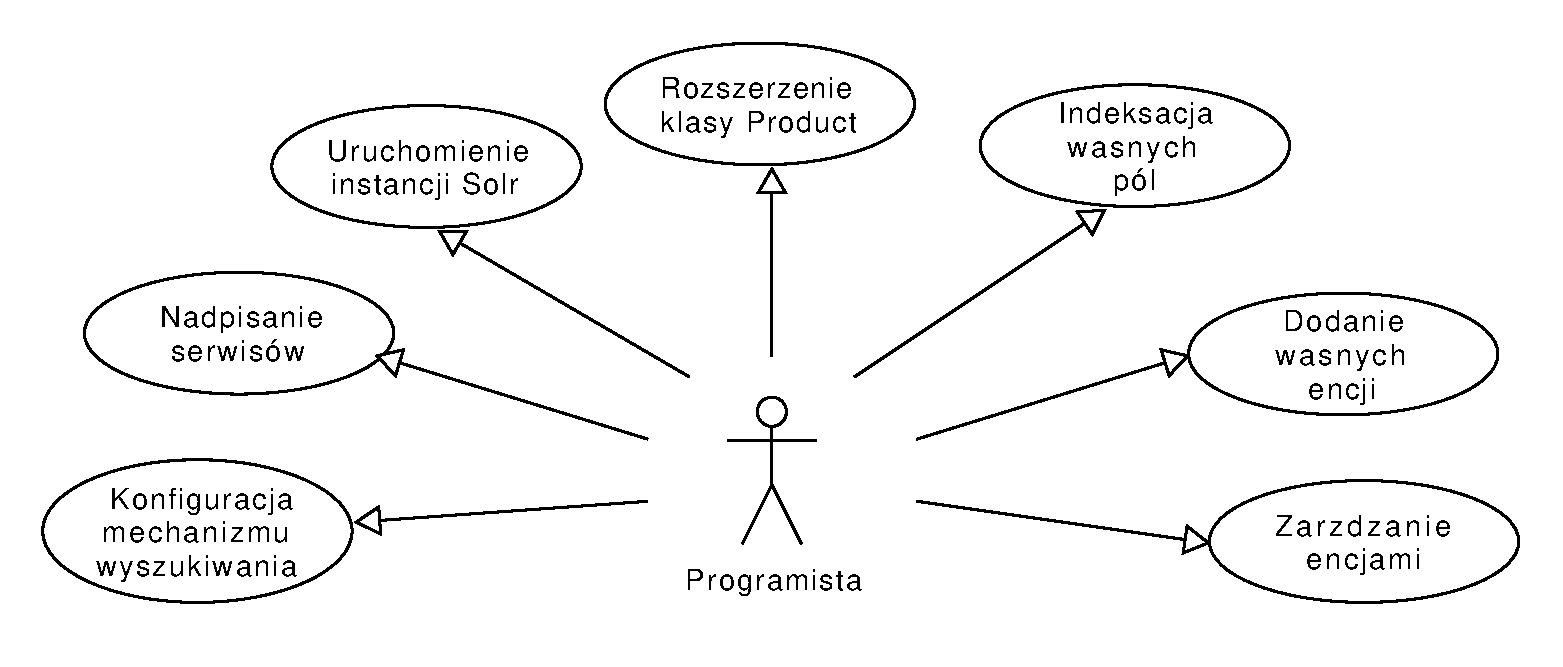
\includegraphics[width=1\textwidth]{ucdev.pdf}
\end{center}
\caption{{\color{black}Diagram przypadków użycia związany z Programistą.}} \label{useCaseProgrammer}
\end{figure}
\begin{figure}
	\begin{center}
		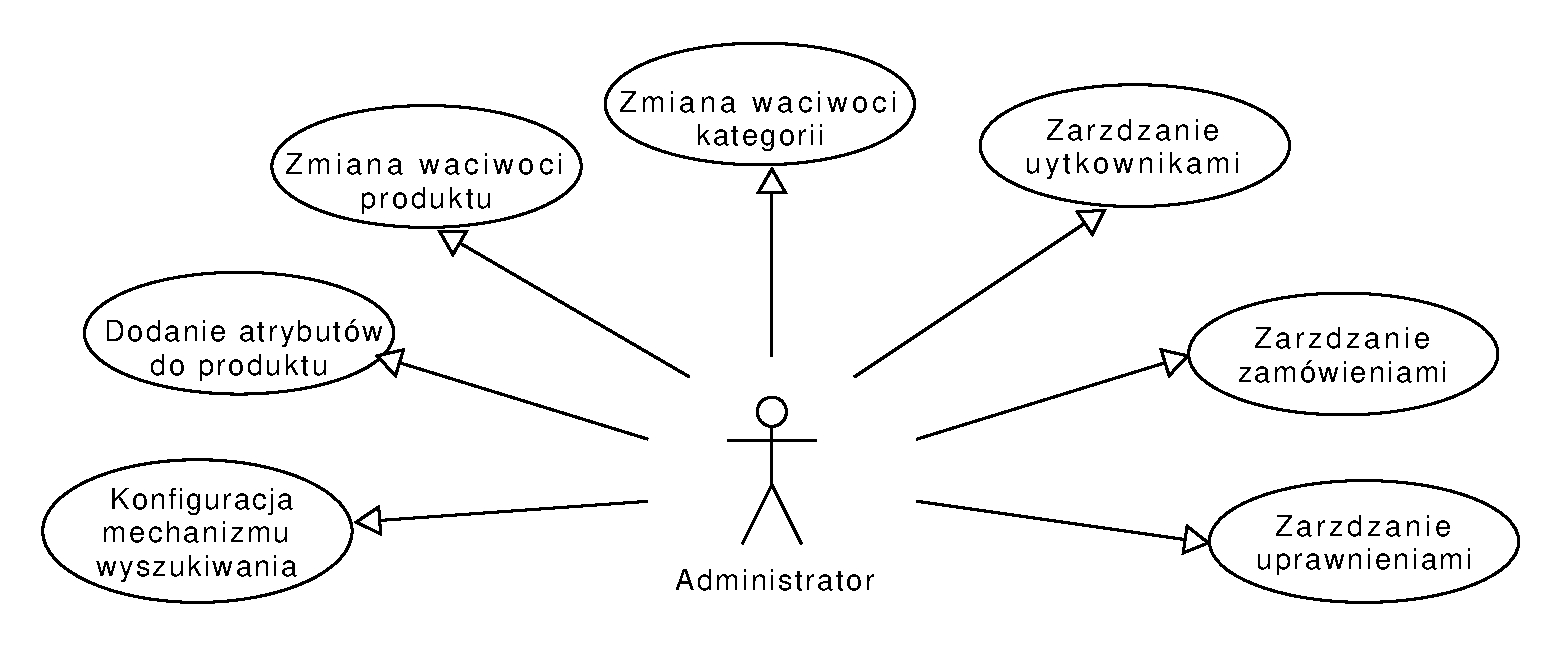
\includegraphics[width=1\textwidth]{ucadmin.pdf}
	\end{center}
	\caption{{\color{black}Diagram przypadków użycia związany z Administratorem ewentualniego systemu.}} \label{useCaseAdmin}
\end{figure}
Rysunek \ref{useCaseAdmin} przedstawia przypadki użycia z punktu widzenia Administratora potencjalnego systemu. Z punktu widzenia platformy jest to również klient, gdyż framework zakłada, że nie ma on wiedzy technicznej i nie potrafi programować. Podobnie jak programista, może konfigurować mechanizm wyszukiwania, jednak bardziej wysokopoziomowo, np. deklaracja używanych facetów. Panel administracyjny zakłada zarządanie najważniejszymi encjami: produkt, kategoria, użytkownik, zamówienie, uprawnienie i parę innych, zdefiniowanych dokładniej w podrozdziale \textbf{Diagramy bazy danych}.

Diagram na rysunku \ref{useCaseCustomer} dotyczy przypadków użycia elementów frameworku przez końcowego użytkownika. Są to klasyczne funkcjonalności tradycyjnego sklepu internetowego. \textit{Wyszukanie produktu} zostało zaprojektowane, tak aby możliwy był również do zaimplementowania mechanizm podpowiedzi i podświetlania. Apache Solr udostępnia taką funkcjonalność. \textit{Reklamacja} dotyczy opisanego w rozdziale \textbf{Analiza problemu} kłopotu z archwizacją produktu, został on rozwiązany prostym mechanizmem wersjonowania. 
\begin{figure}
	\begin{center}
		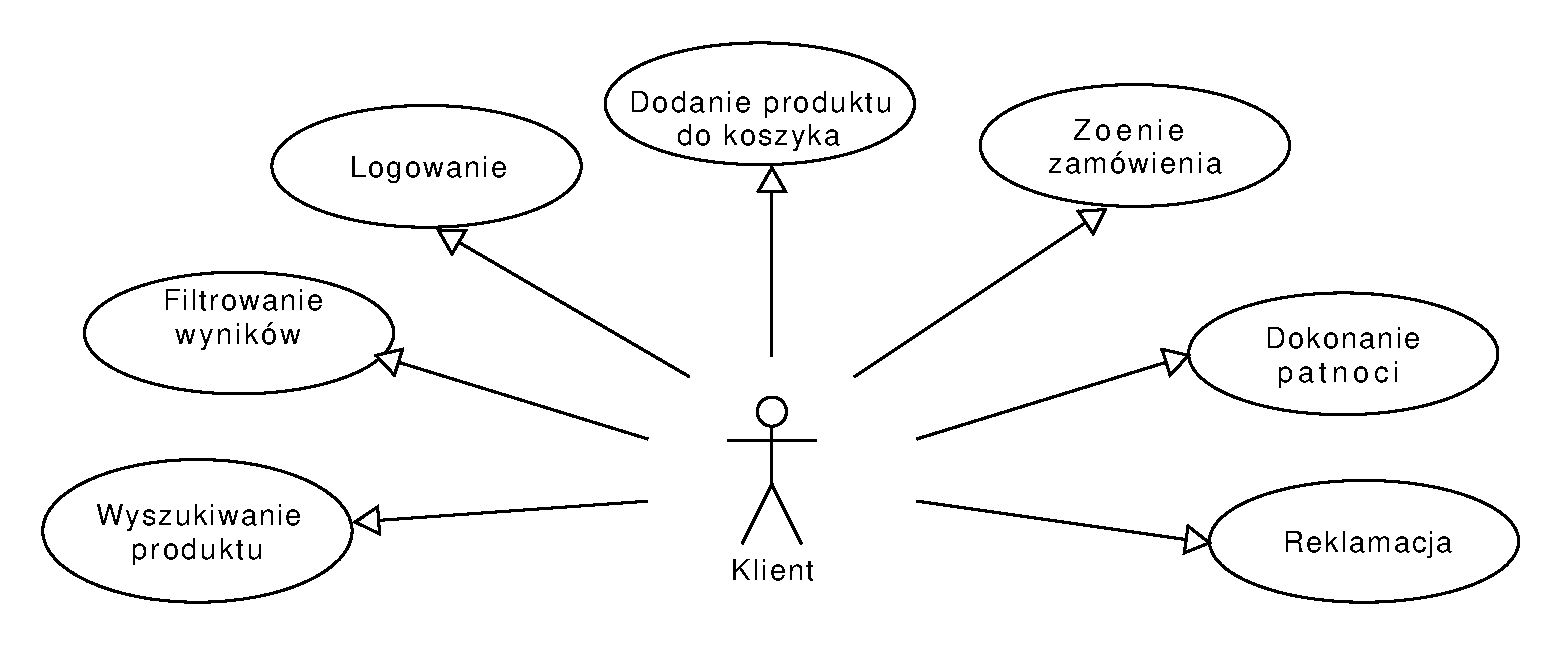
\includegraphics[width=1\textwidth]{uccustomer.pdf}
	\end{center}
	\caption{{\color{black}Diagram przypadków użycia związany z Klientem końcowym ewentualniego systemu.}} \label{useCaseCustomer}
\end{figure}

Diagramy typu \textit{use-case} ściśle wiążą się z wymaganiami funkcjonalnymi systemu. Jest wiadome, że można je również sklasyfikować pod względem aktorów występujących w systemie, dlatego też powiązania przypadków użycia z wymaganiami funkcjonalnymi zostały umieszczone na diagramie z rysunku \ref{wymtoUC}. Na diagram należy patrzeć poziomo, po zapoznaniu się z legendą. Wymagania są w nieprzypadkowej kolejności, są ustawione od lewej do prawej. Im bardziej na prawo, tym wymaganie jest bardziej biznesowe, im bardziej na lewo -- dotyczy rdzeniowych elementów platformy. Warto zauważyć zależność, że im dalej patrzymy na diagram, tym więcej niebieskich i żółtych \textit{use case'ów} -- tych zarezerowowanych dla Administracji i Klientów rozwiązania e-commerce. Natomiast im bardziej na lewo tym więcej czerwonego, czyli przypadków przemyślanych dla Programisty.
\begin{figure}
	\begin{center}
		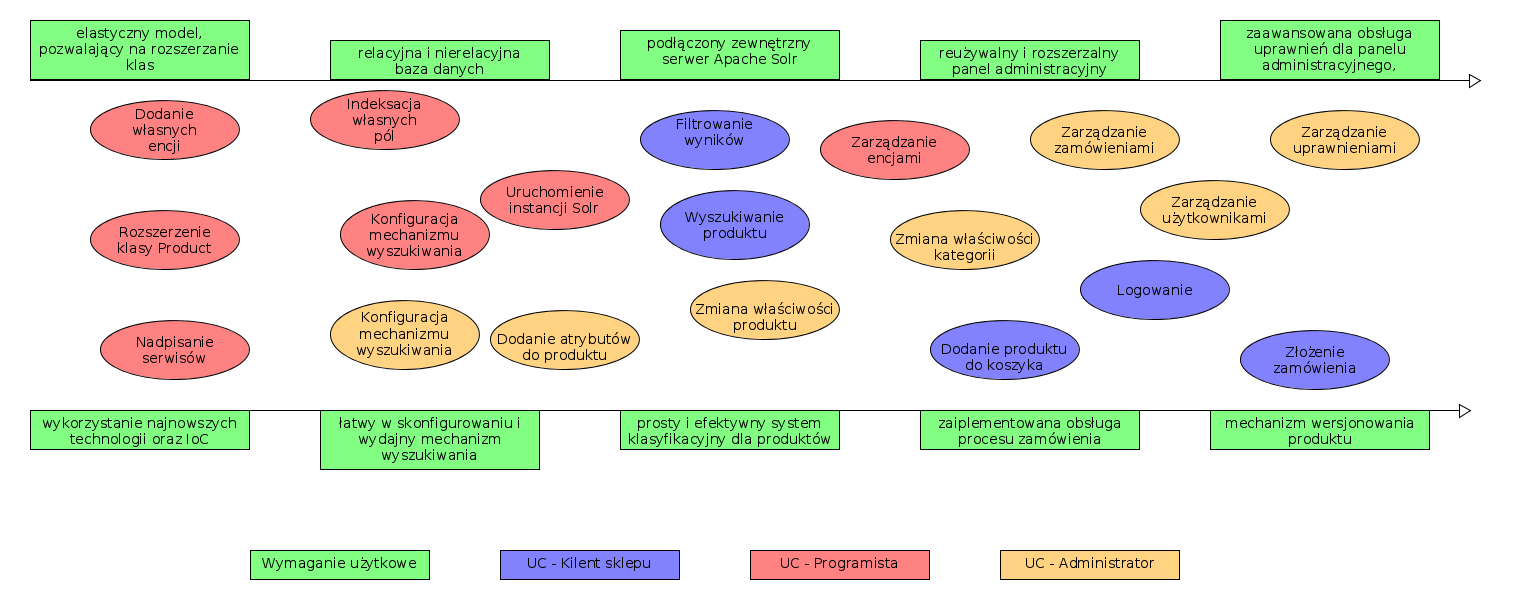
\includegraphics[angle=270,scale=0.4]{wymToUC.png}
	\end{center}
	\caption{{\color{black}Diagram przypadków użycia związany z wymaganiami funkcjonalnymi}} \label{wymtoUC}
\end{figure}

Jak zostało wspomniane wcześniej w sekcji \textbf{Grupy użytkowników i założenia}, framework jest narzędziem głównie dla programisty, to on zdecyduje co ma się znajdować w finalnym systemie, dlatego w niniejszym podrozdziale zostaną rozwinięte przypadki użycia dla programisty związane z obsługą i oprogramowywaniem dynamicznych elementów platformy. Jest to odpowiedź na najtrudniejsze z wymagań, czyli \textbf{elastyczny model, pozwalający na rozszerzenie klas} oraz \textbf{reużywalny i rozszerzalny panel administracyjny}.
\subsection{Dynamiczna tabela encyjna}
Dynamiczna tabela encyjna jest autorskim rozwiązaniem, służącym do wylistowywania dowolnych encji związanych z systemem w panelu administracyjnym, wiążą się z nim przpadki użycia z rysunku \ref{dynEntTabUC}
\begin{figure}[H]
	\begin{center}
		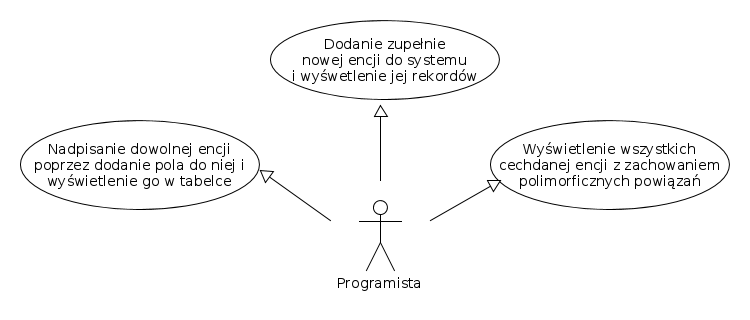
\includegraphics[scale=0.5]{dynEntTabUC.png}
	\end{center}
	\caption{{\color{black}Diagram przypadków użycia związany z dynamiczą tabelą encyjną}} \label{dynEntTabUC}
\end{figure}

\subsection{Dynamiczny formularz encyjny}
Dynamiczny formularz encyjny to kolejne autorskie rozwiązanie, służące do dodawania edycji i wyświetlania szczegółów encji związanych z systemem w panelu administracyjnym, wiążą się z nim przpadki użycia z rysunku \ref{dynEntFormUC}
\begin{figure}[H]
	\begin{center}
		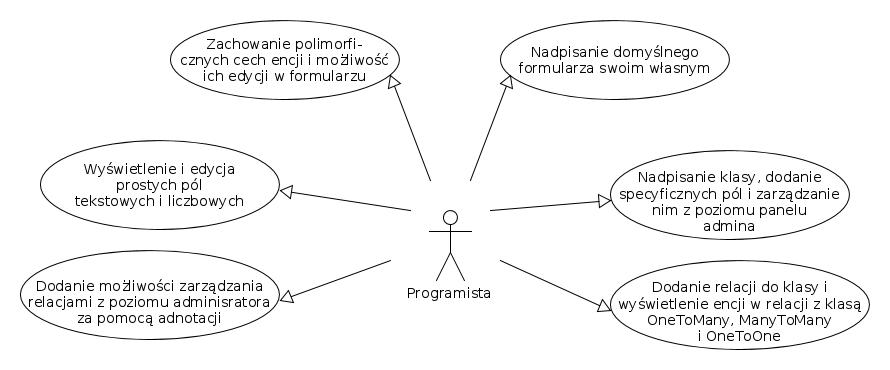
\includegraphics[scale=0.5]{dynEntFormUC.png}
	\end{center}
	\caption{{\color{black}Diagram przypadków użycia związany z dynamicznym formularzem encyjnym}} \label{dynEntFormUC}
\end{figure}

\subsection{Manipulacja produktem}
Produkt w implementowanym systemie jest to encja bardzo dynamiczna, łatwo konfigurowalna. Wiążą się z nim przypadki użycia znajdujące się na rysunku \ref{manipProd}
\begin{figure}[H]
	\begin{center}
		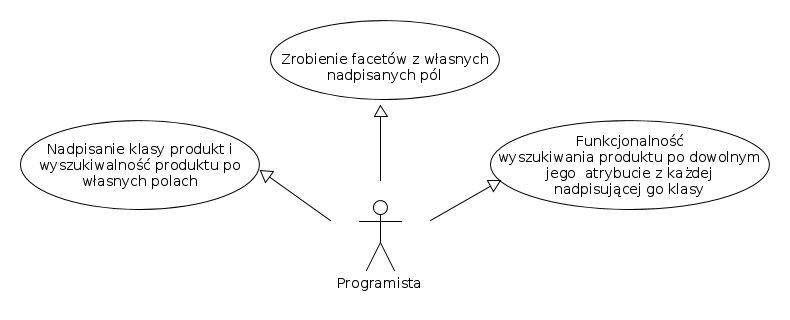
\includegraphics[scale=0.5]{manipProd.png}
	\end{center}
	\caption{{\color{black}Diagram przypadków użycia związany z dynamicznym formularzem encyjnym}} \label{manipProd}
\end{figure}

\section{Diagramy aktywności}
W tej sekcji zostały przedstawione diagramy aktywności dla najbardziej skomplikowanych logicznie elementów systemu. Dynamiczna tabela i formularz opisany w poprzednim punkcie wymagają skomplikowanych operacji aby mogły pozostać ogólne i elastyczne na tyle ile być muszą. Znaczy to, że powinny obsługiwać zmiany w modelu wywołane przez osoby trzecie - \textbf{programistów}. W niniejszym podrozdziale przedstawiono działanie algorytów stojących za dynamicznymi elementami platformy.

\subsection{Wyszukiwanie cech produktu}
Ta sekcja odnosi się do podrozdziału \textbf{Manipulacja produktem}. Wytłumaczono tutaj jak osiągnięto założoną elastyczność przy konfigurowaniu encji reprezentującej produkt w sklepie. 

Każdy Produkt w systemie jest indeksowany, oznacza to że z relacyjnej bazy danych, wraz ze swoimi wszystkimi atrybutami trafia do nierelacyjnych dokumentów na osobnym serwerze, aby odciążyć aplikacje w razie dużego ruchu. Zebranie wszystkich atrybutów produktów to skomplikowane zadanie, gdyż jego cechy mogą być ukryte w następujących miejscach: 
\begin{itemize}
	\item atrybuty dziedziczone po atrybutach klasyfikacyjnych kategorii, w której się znajduje
	\item atrybuty dziedziczone po wszystkich przodkach swojej kategorii
	\item własne pola i pola wszystkich klas, które nadpisały Produkt 
\end{itemize}  

Zadanie to wymaga zejścia do poziomu refleksji w Javie, jednak ten temat został poruszony później. Wyszukiwaniem wszystkich atrybutów obsługuje algorytm, którego diagram aktywności został umieszczony na rysunku \ref{diagramaktywIndeks}

Pierwszym krokiem jest znalezienie wszystkich produktów, co nie jest również oczywistym zadaniem, gdyż nie jest wiadome jaką klasę ma finalny produkt, mógł zostać nadpisany przez programistę, który w swojej klasie zdefiniował pewne pola, które również muszą zostać uwzględnione przy indeksacji produktów. Po znalezieniu \textit{klasy sufitowej} (czyli najwyższej w abstrakcji) mamy pewność, że wszystkie niestandardowe pola znajdą się w obiekcie pobranym przez nas z bazy danych. Z bazy danych muszą zostać również pobrane pola zadeklarowane jako te, które są wyszukiwalne w sklepie (oczywiste jest, że powinno się mieć wybór, które pola z produktu trafią do sklepu, a które nie). Mając te dwie rzeczy, jest możliwe wyciągnąć z obiektu, którego klasa nie jest znana wszystkie interesujące nas pola. Wszystkie wyciągnięte wartości następnie trafiają do dokumentu. Nie jest to jeszcze koniec, gdyż zostają nam jeszcze do wyciągnięcia cechy produktu z systemu klasyfikacyjnego, zostało to zrealizowane algorytmem przejścia po drzewie oraz zapytaniem bazodanowym. Wszystkie cechy produktu są dodawane do listy dokumentów (jeden dokument - jeden produkt) i są wysyłane na serwer Apache Solr. Przykład skąd mogą pochodzić cechy produktu został umieszczone na rysunku \ref{cechyProd}.
\begin{figure}
	\begin{center}
		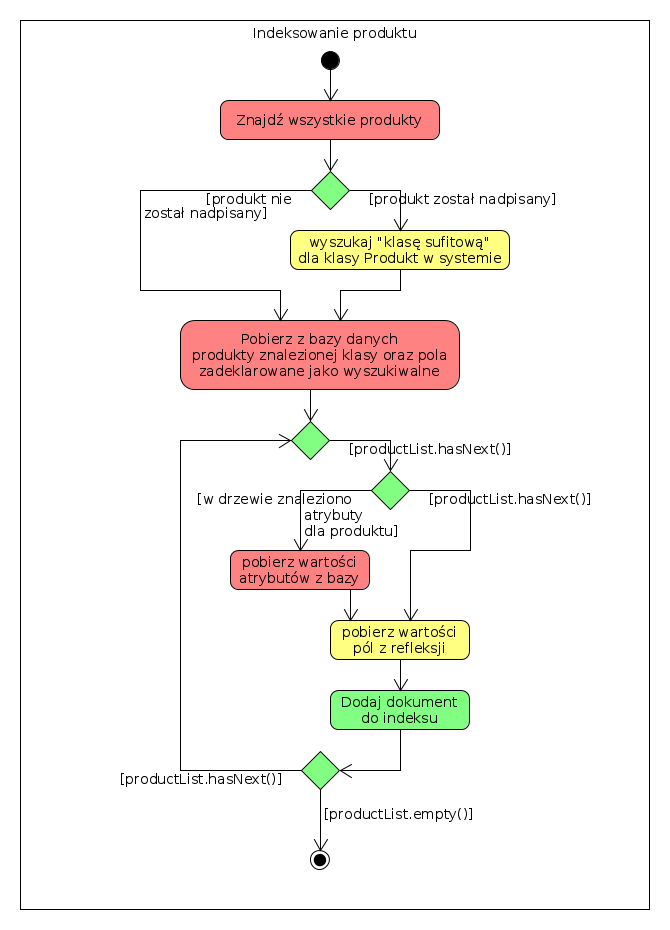
\includegraphics[scale=0.5]{diagramaktywIndeks.png}
	\end{center}
	\caption{{\color{black}Diagram aktywności opisujący algorytm znajodwania wszystkich atrybutów produktu}} \label{diagramaktywIndeks}
\end{figure}
\begin{figure}
	\begin{center}
		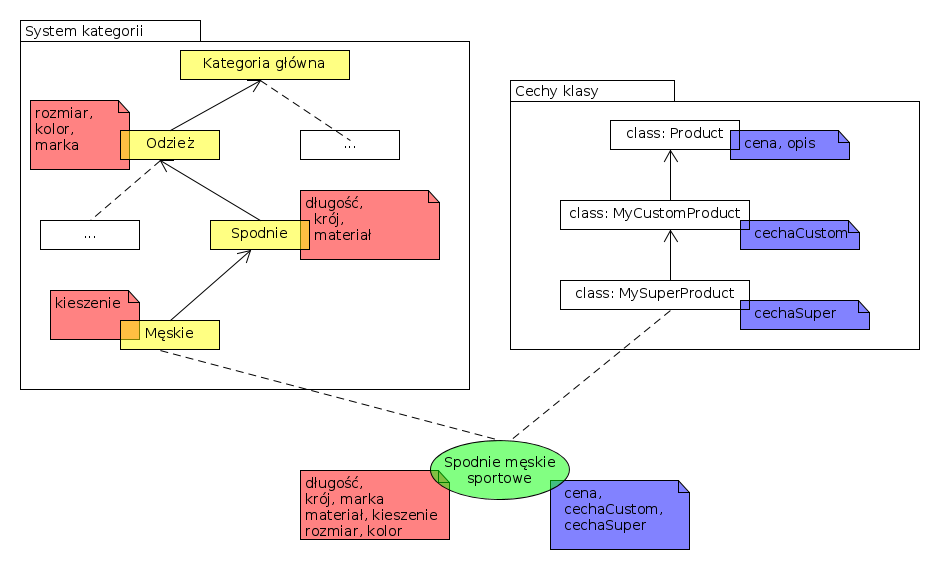
\includegraphics[scale=0.5]{cechyProd.png}
	\end{center}
	\caption{{\color{black}Diagram przykładowy skąd mogą pochodzić cechy produktu}} \label{cechyProd}
\end{figure}

\subsection{Konstrukcja dynamicznej tabeli encyjnej}
Dynamiczna tabela encyjna opisana w poprzednim podrozdziale, jest wbrew pozorom zadaniem analogicznym do wyciągania cech z produktu. Ułatwieniem jest to, że w tabeli nie uwzględnia się atrybutów z systemu klasyfikacyjnego, gdyż dotyczy on tylko produktów, niestety utrudnieniem jest to, że nie jest wiadome jakie klasy dokładnie powinny być wyświetlone w tabelach. Jedyne co jest dane to tabela konfiguracyjna z kodami klas, które mają zostać wyświetlone w panelu administracyjnym. Proces został opisany na diagramie z rysunku \ref{konsTabEnc} 

Najpierw szukane są encje z rodzaju podanego we wspomnianej tablei, następnie refleksją wyciąga się jej pola zaadnotowane przez programistę jako te, które chce wyświetlić w tabeli jako nagłówki (adnotacja \texttt{@AdminVisible(tableVisible=true)}). Ze znalezionej listy obiektów pobiera się wartości pól, które znajdują się w nagłówkach.
\begin{figure}
	\begin{center}
		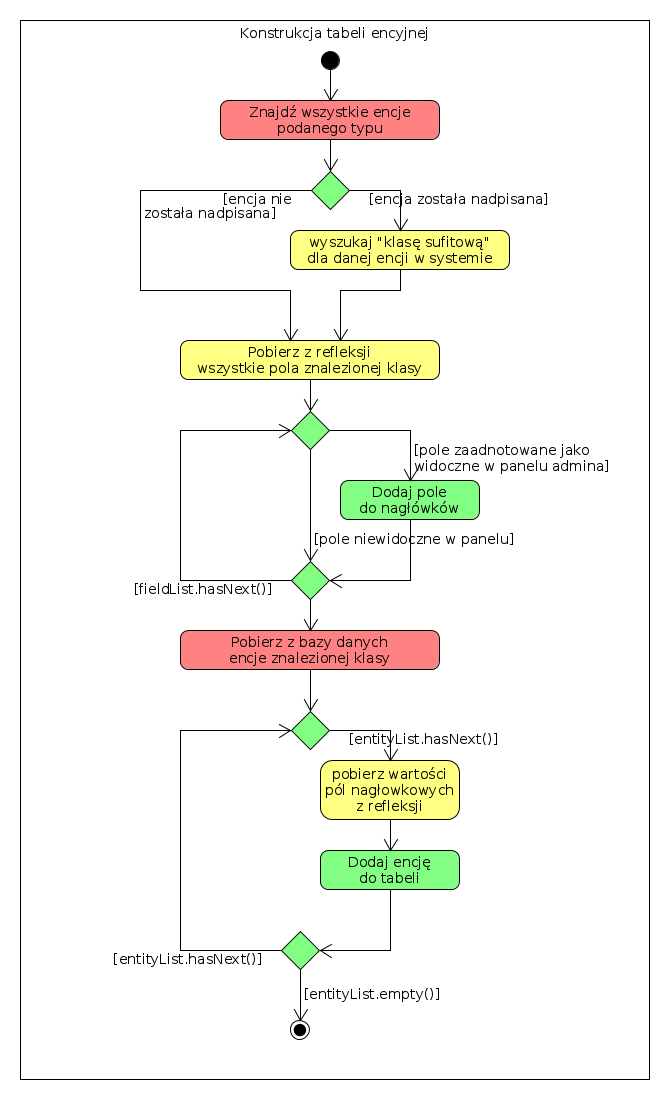
\includegraphics[scale=0.5]{konsTabEnc.png}
	\end{center}
	\caption{{\color{black}Diagram aktywności opisujący algorytm wyszukujący cechy encji uwzględnianych w tabeli.}} \label{konsTabEnc}
\end{figure}

\newpage
\subsection{Konstrukcja dynamicznego formularze encyjnego}
Odbywa się to na bardzo podobnej zasadzie, jak konstrukcja tabeli. Jednak poza polami prostymi zaadnotowanymi jako widzialne w panelu administracyjnym, problem stanowią relacje, które trzeba wyświetlić. Aby zachować rozszerzalność platformie zastosowane zostały tu mechanizmy z dwóch poprzednich przykładów.   

\newpage
\section{Diagramy sekwencji}

W tej sekcji zostały przedstawione diagramy sekwencji dla elementów systemu. Aby zachować spójność w rozważaniach można podzielić je na trzy grupy: 
\begin{itemize}
	\item diagramy dotyczące budowania rozwiązań e-commerce za pomocą platformy
	\item diagramy dotyczące zarządzania rozwiązaniami e-commerce
	\item diagramy dotyczące przebiegu funkcjinalności biznesowych związanych z kientem końcowym
\end{itemize}  
Jak można zauważyć, te trzy grupy korespondują z aktorami opisywanego rozwiązania, zdefiniowanymi na początku rozdziału. Punkt pierwszy dotyczy Programisty, drugi Administratora, a ostatni Klienta końcowego. 


W tej sekcji należy przedstawić diagramy sekwencji dla obiektów systemu zidentyfikowanych na podstawie wcześniejszych rozważań. Należy wykorzystać nazewnictwo wprowadzone w poprzednich rozdziałach, w szczególności odpowiadające definicjom wprowadzonych klas.

\section{Diagramy stanów}

W tej sekcji należy przedstawić diagramy stanów w których może znaleźć się system. Diagramy te są szczególnie istotne przy projektowaniu systemów czasu rzeczywistego. 

\section{Diagramy klas}

W tej sekcji należy przedstawić diagramy klas dla odpowiednich elementów systemu zidentyfikowane na podstawie wcześniejszych rozważań

\section{Projekt bazy danych}

W tej sekcji należy przedstawić projekt bazy danych. Należy omówić wycinek rzeczywistości i odpowiadające mu zidentyfikowane elementy systemu, których wartości będą podlegać utrwalaniu. Należy przedyskutować wybór typów danych dla atrybutów poszczególnych obiektów. Należy uzasadnić wybór platformy DBMS. Dla relacyjnych baz danych należy przedyskutować jej normalizację.

\section{Opis protokołów}

W tej sekcji należy omówić protokoły wykorzystywane przez komponenty systemu. Omówić formaty komunikatów i zilustrować je przykładami. 

\section{Opis algorytmów}

W tej sekcji należy wymienić i przedyskutować algorytmy wykorzystywane w systemie. Algorytmy należy przedstawić w pseudokodzie (wykorzystać pakiet \texttt{algorithm2e}). Omówienia poszczególnych kroków algorytmów powinny zawierać odwołania do odpowiednich linii pseudokodu. Dla zaproponowanych autorskich algorytmów należy przeprowadzić analizę ich złożoności czasowej i pamięciowej. 

{\color{dgray}
Algorytm bąblowania jest przedstawiony w Pseudokodzie~\ref{alg:mine}.
}

{\small
\begin{pseudokod}[H]
%\SetAlTitleFnt{small}
\SetArgSty{normalfont}
\SetKwFunction{Process}{Process}
\SetKwFunction{Calculate}{Calculate}
\KwIn{Zbiór bąbli $B$}
\KwOut{Wyporność $W$}
\ForEach{$b \in B$}{
\Process{$b$}\;
\For{$i \leftarrow 1$ \KwTo $|B|$}{
\If{\Calculate{EW($i$,$b$)} $\le$ 0}{
$b \leftarrow 2*b$\;
}
}
}
\While{$B \neq \emptyset$}{
\For{$j \leftarrow 1$ \KwTo $|B|$}{
\If{\Calculate{FT($j$,$\hat{b}$)} $\le 0$}{
$w \leftarrow 2*\hat{b}$\;
$W \leftarrow W \cup \{w\}$\;
$B \leftarrow B \setminus \{b\}$\;
}
}
}
\caption{Wyporność przez bąblowanie}\label{alg:mine}
\end{pseudokod}
}

